\documentclass{article}\usepackage[]{graphicx}\usepackage[]{color}
%% maxwidth is the original width if it is less than linewidth
%% otherwise use linewidth (to make sure the graphics do not exceed the margin)
\makeatletter
\def\maxwidth{ %
  \ifdim\Gin@nat@width>\linewidth
    \linewidth
  \else
    \Gin@nat@width
  \fi
}
\makeatother

\definecolor{fgcolor}{rgb}{0.345, 0.345, 0.345}
\newcommand{\hlnum}[1]{\textcolor[rgb]{0.686,0.059,0.569}{#1}}%
\newcommand{\hlstr}[1]{\textcolor[rgb]{0.192,0.494,0.8}{#1}}%
\newcommand{\hlcom}[1]{\textcolor[rgb]{0.678,0.584,0.686}{\textit{#1}}}%
\newcommand{\hlopt}[1]{\textcolor[rgb]{0,0,0}{#1}}%
\newcommand{\hlstd}[1]{\textcolor[rgb]{0.345,0.345,0.345}{#1}}%
\newcommand{\hlkwa}[1]{\textcolor[rgb]{0.161,0.373,0.58}{\textbf{#1}}}%
\newcommand{\hlkwb}[1]{\textcolor[rgb]{0.69,0.353,0.396}{#1}}%
\newcommand{\hlkwc}[1]{\textcolor[rgb]{0.333,0.667,0.333}{#1}}%
\newcommand{\hlkwd}[1]{\textcolor[rgb]{0.737,0.353,0.396}{\textbf{#1}}}%

\usepackage{framed}
\makeatletter
\newenvironment{kframe}{%
 \def\at@end@of@kframe{}%
 \ifinner\ifhmode%
  \def\at@end@of@kframe{\end{minipage}}%
  \begin{minipage}{\columnwidth}%
 \fi\fi%
 \def\FrameCommand##1{\hskip\@totalleftmargin \hskip-\fboxsep
 \colorbox{shadecolor}{##1}\hskip-\fboxsep
     % There is no \\@totalrightmargin, so:
     \hskip-\linewidth \hskip-\@totalleftmargin \hskip\columnwidth}%
 \MakeFramed {\advance\hsize-\width
   \@totalleftmargin\z@ \linewidth\hsize
   \@setminipage}}%
 {\par\unskip\endMakeFramed%
 \at@end@of@kframe}
\makeatother

\definecolor{shadecolor}{rgb}{.97, .97, .97}
\definecolor{messagecolor}{rgb}{0, 0, 0}
\definecolor{warningcolor}{rgb}{1, 0, 1}
\definecolor{errorcolor}{rgb}{1, 0, 0}
\newenvironment{knitrout}{}{} % an empty environment to be redefined in TeX

\usepackage{alltt}
\usepackage{graphicx, color, hyperref, fancyhdr}

%\usepackage{amsmath,amssymb,amsthm}
\usepackage{fancyhdr,url}
\usepackage{graphicx}

\oddsidemargin 0in  %0.5in
\topmargin     0in
\leftmargin    0in
\rightmargin   0in
\textheight    9in
\textwidth     6in %6in
%\headheight    0in
%\headsep       0in
%\footskip      0.5in

\newtheorem{thm}{Theorem}
\newtheorem{cor}[thm]{Corollary}
\newtheorem{obs}{Observation}
\newtheorem{lemma}{Lemma}
\newtheorem{claim}{Claim}
\newtheorem{definition}{Definition}
\newtheorem{question}{Question}
\newtheorem{answer}{Answer}
\newtheorem{problem}{Problem}
\newtheorem{solution}{Solution}
\newtheorem{conjecture}{Conjecture}

\pagestyle{fancy}

\lhead{\textsc{MATH 243}}
\chead{\textsc{Practice}}
\rhead{\textsc{\today}}
\lfoot{}
\cfoot{}
%\cfoot{\thepage}
\rfoot{}
\renewcommand{\headrulewidth}{0.2pt}
\renewcommand{\footrulewidth}{0.0pt}

\newcommand{\ans}{\vspace{0.25in}}

\usepackage[top=.5in, bottom=.5in, left=1.1in, right=1.1in]{geometry}
\thispagestyle{empty}
\IfFileExists{upquote.sty}{\usepackage{upquote}}{}
\begin{document}

\begin{center}
\textsc{Math 243: Statistical Learning} \\
\noindent\rule{12cm}{0.4pt}
\end{center}

\begin{minipage}{.5\linewidth}
{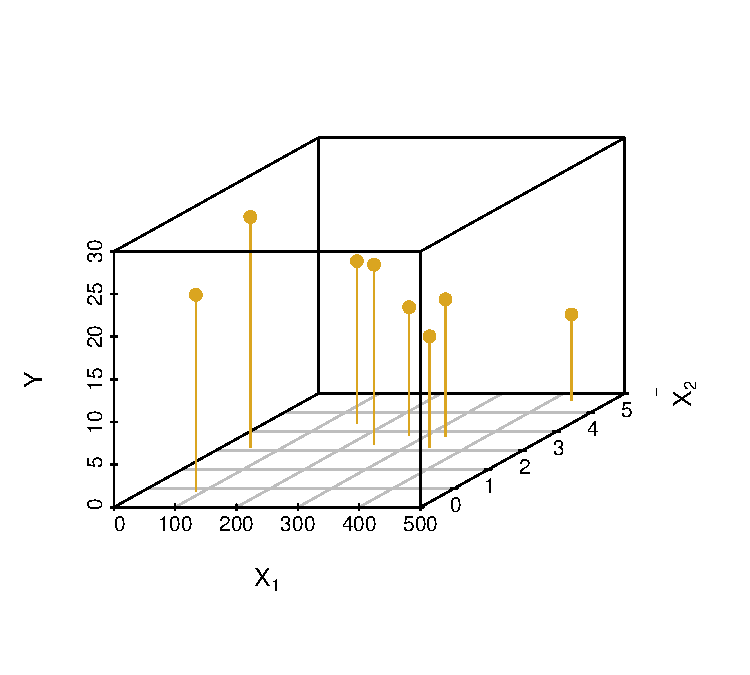
\includegraphics[scale=0.6]{scatterA.pdf}}
\end{minipage}

\begin{minipage}{.5\linewidth}
jk
\end{minipage}

NULL
% latex table generated in R 3.2.3 by xtable 1.8-2 package
% Tue Mar 29 23:20:10 2016
\begin{table}[ht]
\centering
\begin{tabular}{rrrrll}
  \hline
 & X1 & X2 & Y & $\hat{f}^1(x)$ & r \\ 
  \hline
1 & 288.09 & 3.81 & 16.00 &  &  \\ 
  2 & 86.03 & 0.86 & 23.00 &  &  \\ 
  3 & 149.53 & 4.44 & 19.00 &  &  \\ 
  4 & 331.15 & 3.77 & 16.00 &  &  \\ 
  5 & 430.89 & 5.68 & 10.00 &  &  \\ 
  6 & 338.36 & 3.18 & 13.00 &  &  \\ 
  7 & 46.33 & 3.17 & 27.00 &  &  \\ 
  8 & 238.19 & 3.35 & 21.00 &  &  \\ 
   \hline
\end{tabular}
\end{table}


\begin{table}[ht]
\centering
\begin{tabular}{rrrrr}
  \hline
 & $\hat{f}^1(x)$ & $\hat{f}^2(x)$ & $\hat{f}^3(x)$ & $\hat{f}^{boost}(x)$\\ 
  \hline
1 & & & &  \\ 
2 & & & & \\ 
3 & & & &  \\ 
4 & & & &  \\ 
5 & & & &  \\ 
6 & & & &  \\ 
7 & & & & \\ 
8 & & & &  \\ 
   \hline
\end{tabular}
\end{table}

\end{document}
